\documentclass{article}
    % General document formatting
    \usepackage[margin=0.7in]{geometry}
    \usepackage{amsthm}
    \usepackage[parfill]{parskip}
    \usepackage[utf8]{inputenc}
    \usepackage{cancel}
    \usepackage{graphicx}
    \usepackage[danish]{babel}
    \usepackage{mathtools}

    \graphicspath{./skitser/}
    % Related to math
    \usepackage{amsmath,amssymb,amsfonts,amsthm}

\makeatletter
\newenvironment{proofw}{\par
  \pushQED{\qed}%
  \normalfont \topsep6\p@\@plus6\p@\relax
  \trivlist
  \item[]\ignorespaces
}{%
  \popQED\endtrivlist\@endpefalse
}
\makeatother

\begin{document}

\tableofcontents

\section{Vektorer og trigonometri}

\subsection{Bevis}

\begin{proofw}
    
Betragt figur \ref{fig:trekant_vektor}, hvor en vinkel $v$ er udspændt af vektoren $\vec{x}$ og $\vec{y}$.

\begin{figure}[h]
    \centering
    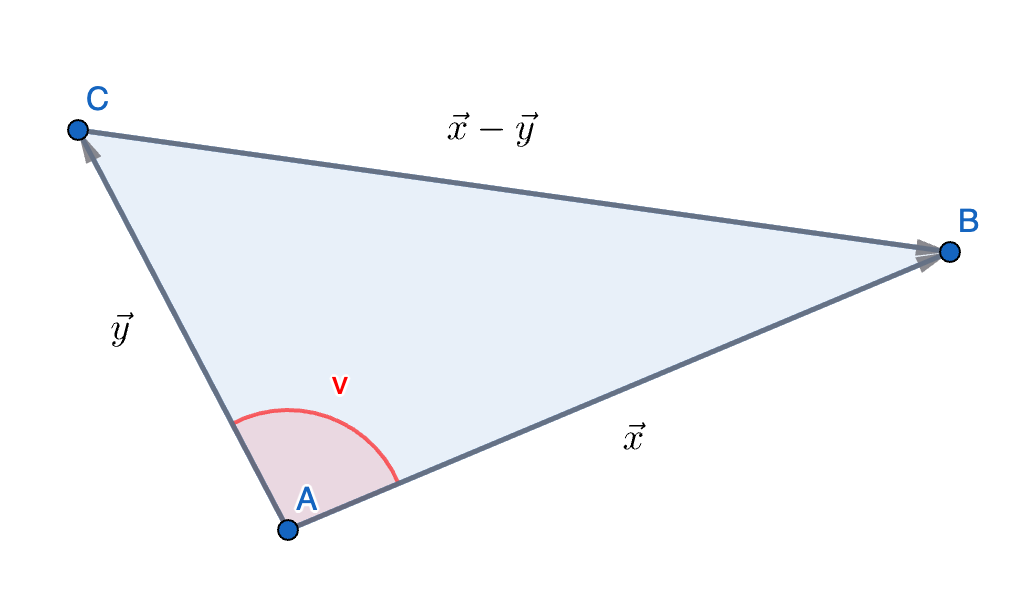
\includegraphics[scale=0.3]{./skitser/trekant_vektor_skitse.png}
    \label{fig:trekant_vektor}
    \caption{Vinkel udspændt af 2 vektorer.}
\end{figure}

Vha. af disse vektorer kan vi danne en trekant, hvori vi kan anvende cosinusrelationerne
til at lave et generelt udtryk for vinklen udspændt af 2 vektorer.
Her kan vi lave et udtryk for den lange side ved at anvende indskudsreglen:

\begin{align*}
    \vec{AB}+\vec{BC}&=\vec{AC}
    \\
    &\Downarrow
    \\
    \vec{BC}&=\vec{AC}-\vec{AB}
    \\
    &\Downarrow
    \\
    \vec{CB}&=-\vec{BC}=\vec{AB}-\vec{AC}
\end{align*}

Så den trejde side noteres $\vec{x}-\vec{y}$, og vi anvender cosinusrelationen, der siger, at i en trekant, så:

$$
    c^2=a^2+b^2-2ab \cdot \cos(v)
$$

Hvilket i vores tilfælde betyder:

$$
    |\vec{x}-\vec{y}|^2=|\vec{x}|^2+|\vec{y}|^2-2|\vec{x}||\vec{y}| \cdot \cos(v)
$$

Nu anvendes det, at $|\vec{x}|^2=\vec{x} \cdot \vec{x}$, det betyder for vores vektor:

$$
    |\vec{x}-\vec{y}|^2=(\vec{x}-\vec{y})\cdot (\vec{x}-\vec{y})
    =|\vec{x}|^2+|\vec{y}|^2-2 \cdot \vec{x}\cdot \vec{y}
$$

Det indsættes i ovenstående:

$$
\cancel{|\vec{x}|^2+|\vec{y}|^2-2} \cdot \vec{x}\cdot \vec{y}
=\cancel{|\vec{x}|^2+|\vec{y}|^2-2}|\vec{x}||\vec{y}| \cdot \cos(v)
$$

Hvor $\cos(v)$ isoleres:

$$
    \cos(v)=\frac{
        \vec{x} \cdot \vec{y}
    }{
        |\vec{x}||\vec{y}|
    }
$$
\end{proofw}

\section{Vektorer og linjer i planen}

\subsection{Bevis af linjens parameterfremstilling}

\begin{proofw}
    Betragt følgende skitse:
    \begin{figure}[h]
        \centering
        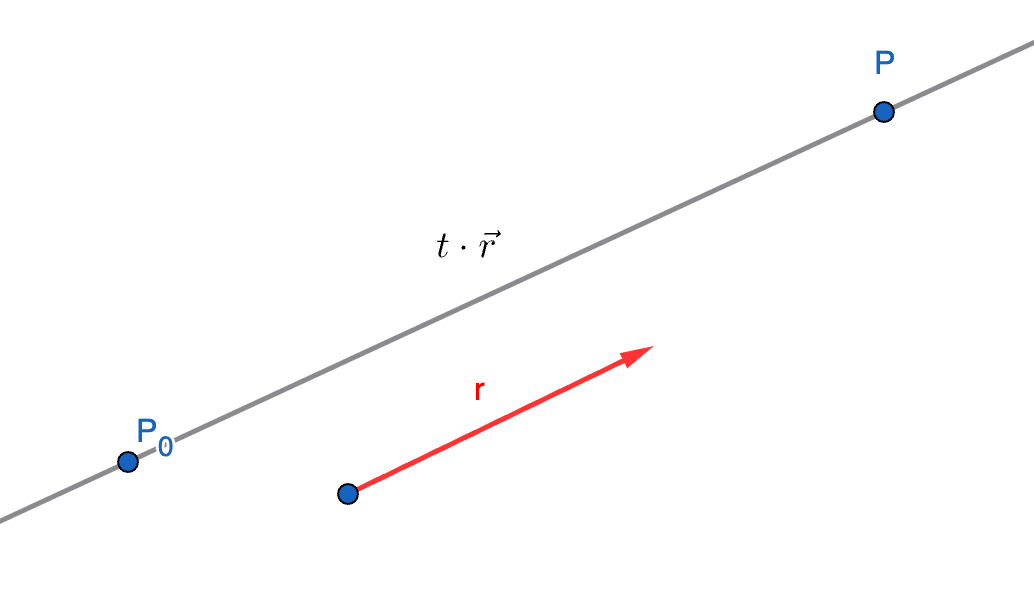
\includegraphics[scale=0.4]{skitser/linje_parameter.png}
    \end{figure}

Tager vi afsæt i punktet $P_0(x_0,y_0)$, hvis position kan beskrives
med vektoren $\vec{OP}$. Tager vi et skridt langs en vektor, der er parallel med linjen,
så vil vores nye position også være på linjen.
Derfor må vi ved at gange retningsvektoren med et vilkårligt tal
kunne ramme alle punkter på linjen.
Så kan vi beskrive vektoren til punktet $P(x,y)$
som vektoren til $P_0$ plus retningsvektoren skaleret:

$$
\vec{OP}=\vec{OP_0}+t\cdot \vec{r}
$$

Vi opsplitter $\vec{OP}$ i $\begin{pmatrix}
    x \\ y
\end{pmatrix}$ og $\vec{r}$ i $\begin{pmatrix}
    r_1 \\ r_2
\end{pmatrix}$:

$$
\begin{pmatrix}
    x
    \\
    y
\end{pmatrix}
=\begin{pmatrix}
    x_0
    \\
    y_0
\end{pmatrix}
+
t \cdot \begin{pmatrix}
    r_1
    \\
    r_2
\end{pmatrix}
$$
\end{proofw}

\subsection{Bevis af linjens ligning}

\begin{proofw}
    Betragt nedenstående figur:
    \begin{figure}[h]
        \centering
        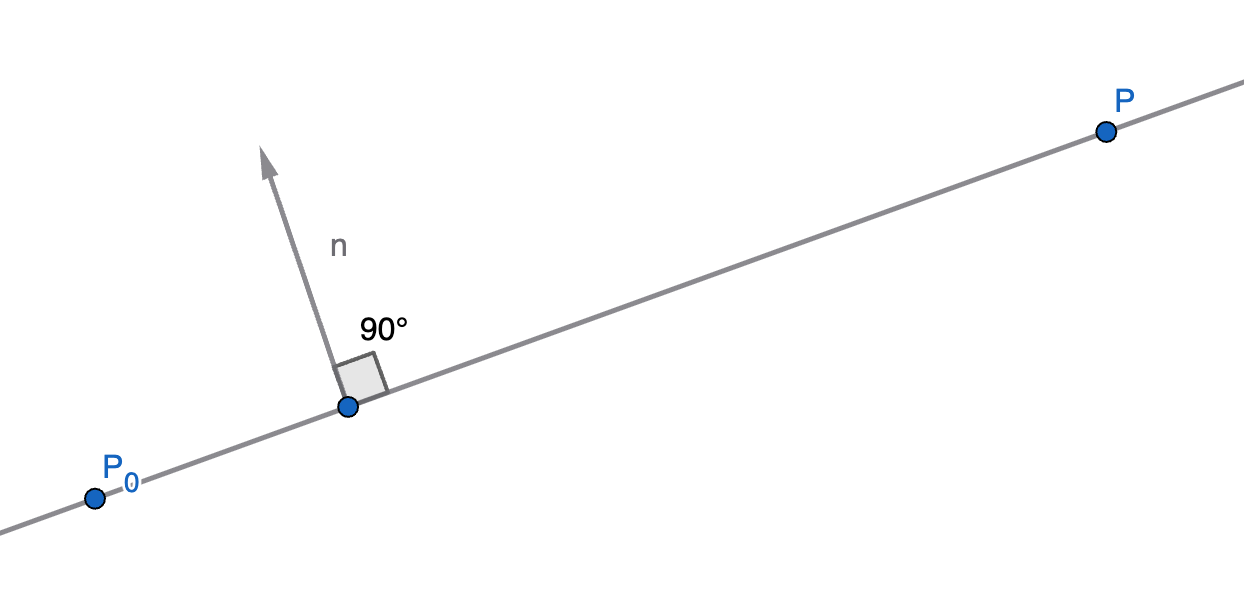
\includegraphics[scale=0.4]{skitser/linjens_ligning.png}
    \end{figure}

    Vi kender $P_0(x_0,y_0)$ og normalvektoren $\vec{n}=\begin{pmatrix}
        a \\ b
    \end{pmatrix}$, $P(x,y)$ er et vilkårligt punkt langs linjen, som vi vil beskrive.
    Vi kan lave en ortogonal vektor til $\vec{n}$ ved at lave vektoren $\vec{P_0P}=\begin{pmatrix}
        x-x_0
        \\
        y-y_0
    \end{pmatrix}$.
    Tricket er så, at vi har 2 ortogonale vektorer, hvilket betyder,
    at deres skalarprodukt er 0, derved kan vi opstille følgende udtryk, hvor $x$ og $y$ alle er punkter på linjen:

    \begin{align*}
        \vec{P_0P}&\cdot\vec{n}=0
        \\
        &\Downarrow
        \\
        \begin{pmatrix}
            x-x_0
            \\
            y-y_0
        \end{pmatrix}
        &\cdot
        \begin{pmatrix}
            a \\
            b
        \end{pmatrix}=0
        \\
        \Downarrow
        \\
        a(x-x_0)&+b(y-y_0)=0
        \\
        \Downarrow
        \\
        ax+by+&(-ax_0-by_0)=0
        \\
        \Downarrow
        \\
        ax+by&+c=0
    \end{align*}

    Det er vist, at en linje kan beskrives ud fra et punkt og en normalvektor til linjen.

\end{proofw}

\section{Vektorer og vektorfunktioner}

\subsection{Bevis af cirklens parameterfremstilling}

\begin{proofw}
    \begin{figure}[h]
        \centering
        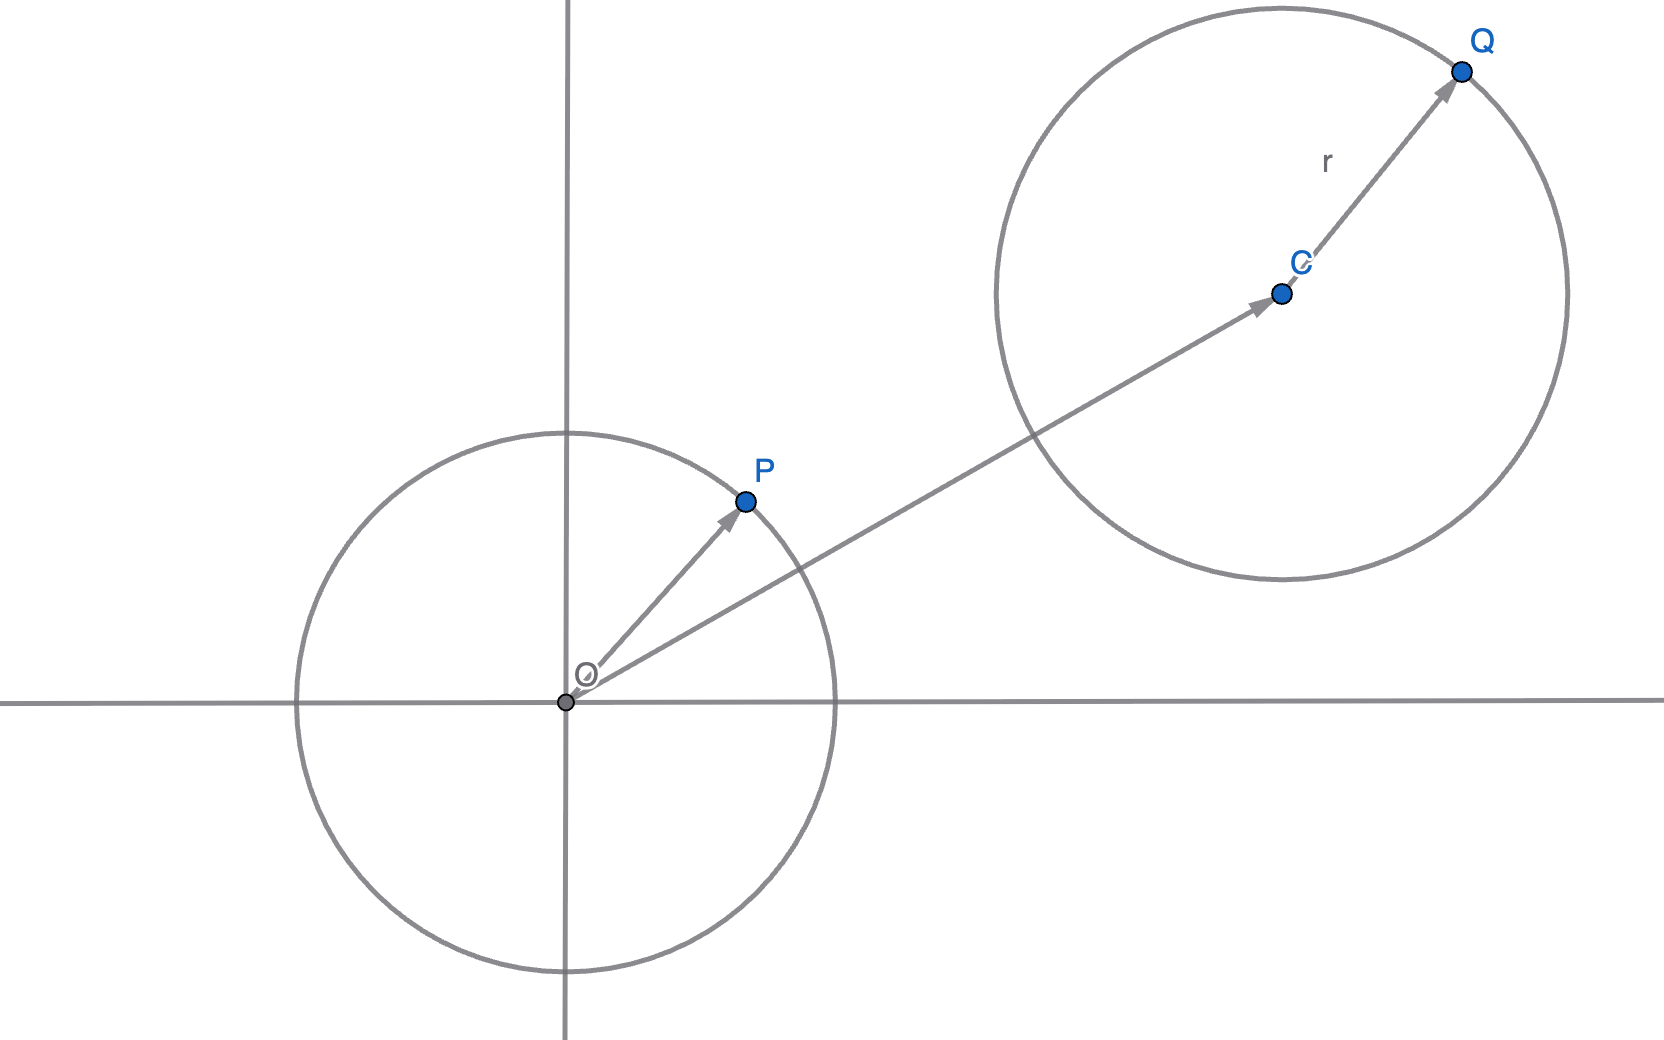
\includegraphics[scale=0.3]{skitser/cirkel.png}
    \end{figure}

    Betragt ovenstående figur, først tager vi tilfældet,
    hvor cirklen har centrum i origo. Her vil alle punkter
    på cirkelperifirien kunne beskrives som en skalering af enhedscirklen, derfor:

    $$
        \vec{OP}=\begin{pmatrix}
            r\cdot \cos(t)
            \\
            r\cdot \sin(t)
        \end{pmatrix}
    $$
    
    For cirklen, der ikke har centrum i origo, er situationen en smule anderledes,
    men vektoren $\vec{CQ}=\vec{OP}$, da cirklerne har samme radius $r$.
    Vi anvender indskudsreglen til at finde:

    $$
        \vec{OQ}=\vec{OC}+\vec{CQ}
    $$

    Disse værdier kender vi, så parameterfremstillingen bliver:

    $$
    \begin{pmatrix}
        x \\ y
    \end{pmatrix}
    =\begin{pmatrix}
        a \\ b
    \end{pmatrix}
    +
    \begin{pmatrix}
        r \cdot \cos(t)
        \\
        r \cdot \sin(t)
    \end{pmatrix}
    =\begin{pmatrix}
        a+ r \cdot \cos(t)
        \\
        b+ r \cdot \sin(t)
    \end{pmatrix}
    $$

\end{proofw}

\section{Funktioner og differentialregning}

Den naturlige eksponential funktion er defineret som Eulers tal $e$ opløftet i $x$:

$$f(x)=e^x$$

Den har samme egenskab som alle andre eksponentielle funktioner, at den går gennem $(0,1)$.
Det som gør den speciel er, at dens hældning også er $1$ i $(0,1)$.

\subsection{Bevis af differentialkvotienten for den naturlige eksponentialfunktion}
\begin{proofw}
    Vi anvender, at $f'(0)=1$, da vi kan opskrive differenskvotienten i $0$ som:

    $$
    \lim_{h \rightarrow 0}
    \frac{e^h-1}{h}=1
    $$

    Vi kan også opskrive differenskvotienten for et vilkårligt punkt:

    $$
        \frac{\Delta y}{h}=\frac{e^{x_0+h}-e^{x_0}}{h}=e^{x_0}\cdot \frac{e^h-1}{h}
    $$

    Når vi lader $h \rightarrow 0$, så:

    $$
       f'(x)= \lim_{h \rightarrow 0} e^{x_0} \cdot \frac{e^h-1}{h}=e^{x_0} \cdot 1=e^{x_0}
    $$

    Derved er det bevist, at $\frac{\partial}{\partial x} e^x=e^x$.
\end{proofw}

\section{Funktioner og differentialregning}

\subsection{Bevis af produktreglen}

\begin{proofw}
    

Vi har 2 funktioner $f$ og $g$, og vi vil finde den afledte af deres produktfunktion, dvs.:

$$
    (f\cdot g)'(x)
$$

For hver funktion kan vi opstille en differenskvotient, som bliver til differentialkvotienter, når vi lader $h \rightarrow 0$:

$$
    \frac{f(x+h)-f(x)}{h} \xrightarrow[h \rightarrow 0]{} f'(x)
$$

$$
    \frac{g(x+h)-g(x)}{h} \xrightarrow[h \rightarrow 0]{} g'(x)
$$

Så opskriver vi differenskvotienten for funktionen $(f \cdot g)(x)$:

$$
    \frac{
        f(x+h)\cdot g(x+h)
        -
        f(x) \cdot g(x)
    }{h}
$$

Så lægger vi $f(x) \cdot g(x+h)$ til og trækker det fra:

$$
    \frac{
        f(x+h)\cdot g(x+h)
        -
        f(x) \cdot g(x+h)
        +
        f(x) \cdot g(x+h)
        -
        f(x) \cdot g(x)
    }{h}
$$

Det ses, at $g(x+h)$ og $f(x)$ kan sættes udenfor parentes:

$$
    \frac{
        g(x+h) \cdot (f(x+h)
        -
        f(x))
        +
        f(x) \cdot (g(x+h)
        -
     \cdot g(x))
    }{h}
$$

Vi opsplitter brøken i 2, og sætter $g(x+h)$ og $f(x)$ udenfor brøkerne:

$$
    g(x+h) \cdot \frac{
          f(x+h)
        -
        f(x)   
    }{h}
    +
        f(x) \cdot 
        \frac{g(x+h)
        -
      g(x)}{h}
$$

Så lader vi $h \rightarrow 0$:

$$
    g(x) \cdot f'(x)+f(x) \cdot g'(x)
$$

Så:

$$
    (f \cdot g)'(x)=    g(x) \cdot f'(x)+f(x) \cdot g'(x)
$$

\end{proofw}

\section{Funktioner i to variable og differentialregning}

\subsection{Bevis af tangentplanens ligning}

\begin{proofw}

Betragt følgende skitse:

\begin{figure}[h]
    \centering
    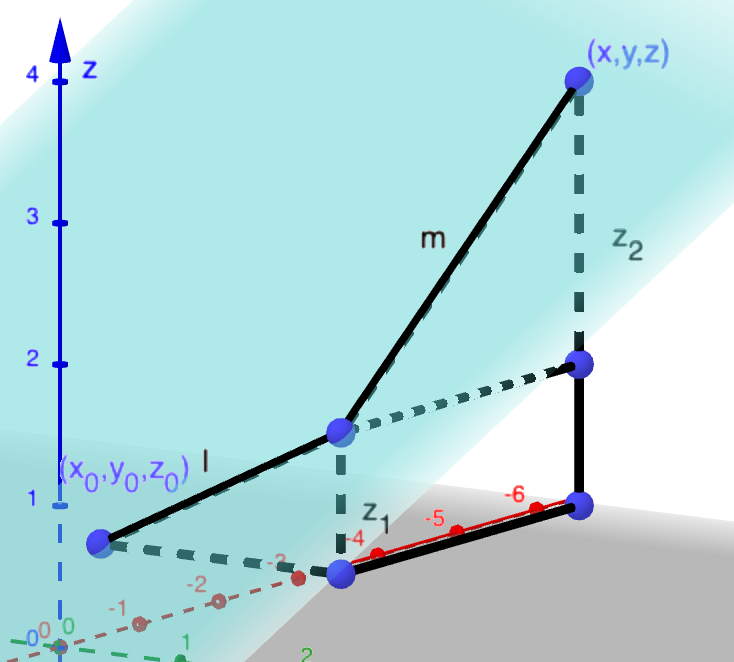
\includegraphics[scale=0.5]{skitser/tangent_plan.png}
\end{figure}

På skitsen er et plan, der følger linjerne $l$ og $m$.
Noterer vi hældningen af $l$ som $p$ og hældningen af $m$ som $q$,
så kan vi opstille følgende udtryk for ændringen på $z$-aksen:

$$
    \Delta z_1=p \cdot (x-x_0)
$$

$$
    \Delta z_2=q \cdot (y-y_0)
$$

Derfor må den nye funktionsværdi $z$ i punktet $(x,y,z)$ være:

$$
    z=z_0+\Delta z_1+\Delta z_2=p \cdot (x-x_0)+q \cdot (y-y_0) + z_0
$$

Det vil sige, at alle $(x,y,z)$, der gør nedenstående ligning sand, er punkter i planet tilhørende
linje $l$ og $m$ med afsæt i punkt $(x_0,y_0,z_0)$:

$$
z=p \cdot (x-x_0)+q \cdot (y-y_0) + z_0
$$

Det ovenstående er dog blot for det generelle plan.
For en tangent plan, som viser hældningen af en funktion af 2 variable,
kan hældningen langs $x$-aksen beskrives som $f_x'(x_0,y_0)$
og langs $y$-aksen $f_y'(x_0,y_0)$.
Sidst kan $z_0$ beskrives som $f(x_0,y_0)$, derfor:

$$
    z=f_x'(x_0,y_0)(x-x_0)+
    f_y'(x_0,y_0)(y-y_0)+
    f(x_0,y_0)
$$

Dette er ligningen for tangentplanet for en funktion af 2 variable.

\end{proofw}

\section{Integralregning og stamfunktioner}

\subsection{Bevis af at alle stamfunktioner til $f(x)$ er på form $F(x)+k$}

\begin{proofw}
    Først vises det, at $F(x)+k$ er en stamfunktion til $f(x)$ da:

    $$
        (F(x)+k)'=F'(x)+k'=f(x)
    $$

    Så vil vi vise, at en anden funktion $G(x)=F(x)+k$ også er stamfunktion,
    da differensfunktionen mærket er 0:

    $$
        (G(x)-F(x))'=F'(x)+k'-F'(x)=f(x)-f(x)=0
    $$

    Derfor:

    $$
        G(x)-F(x)=k \Leftrightarrow G(x)=F(x)+k
    $$

\end{proofw}

\section{Integralregning og arealer}

\subsection{Bevis af at arealfunktionen er stamfunktionen}

\begin{proofw}
    
Betragt følgende skitse:

\begin{figure}[h]
    \centering
    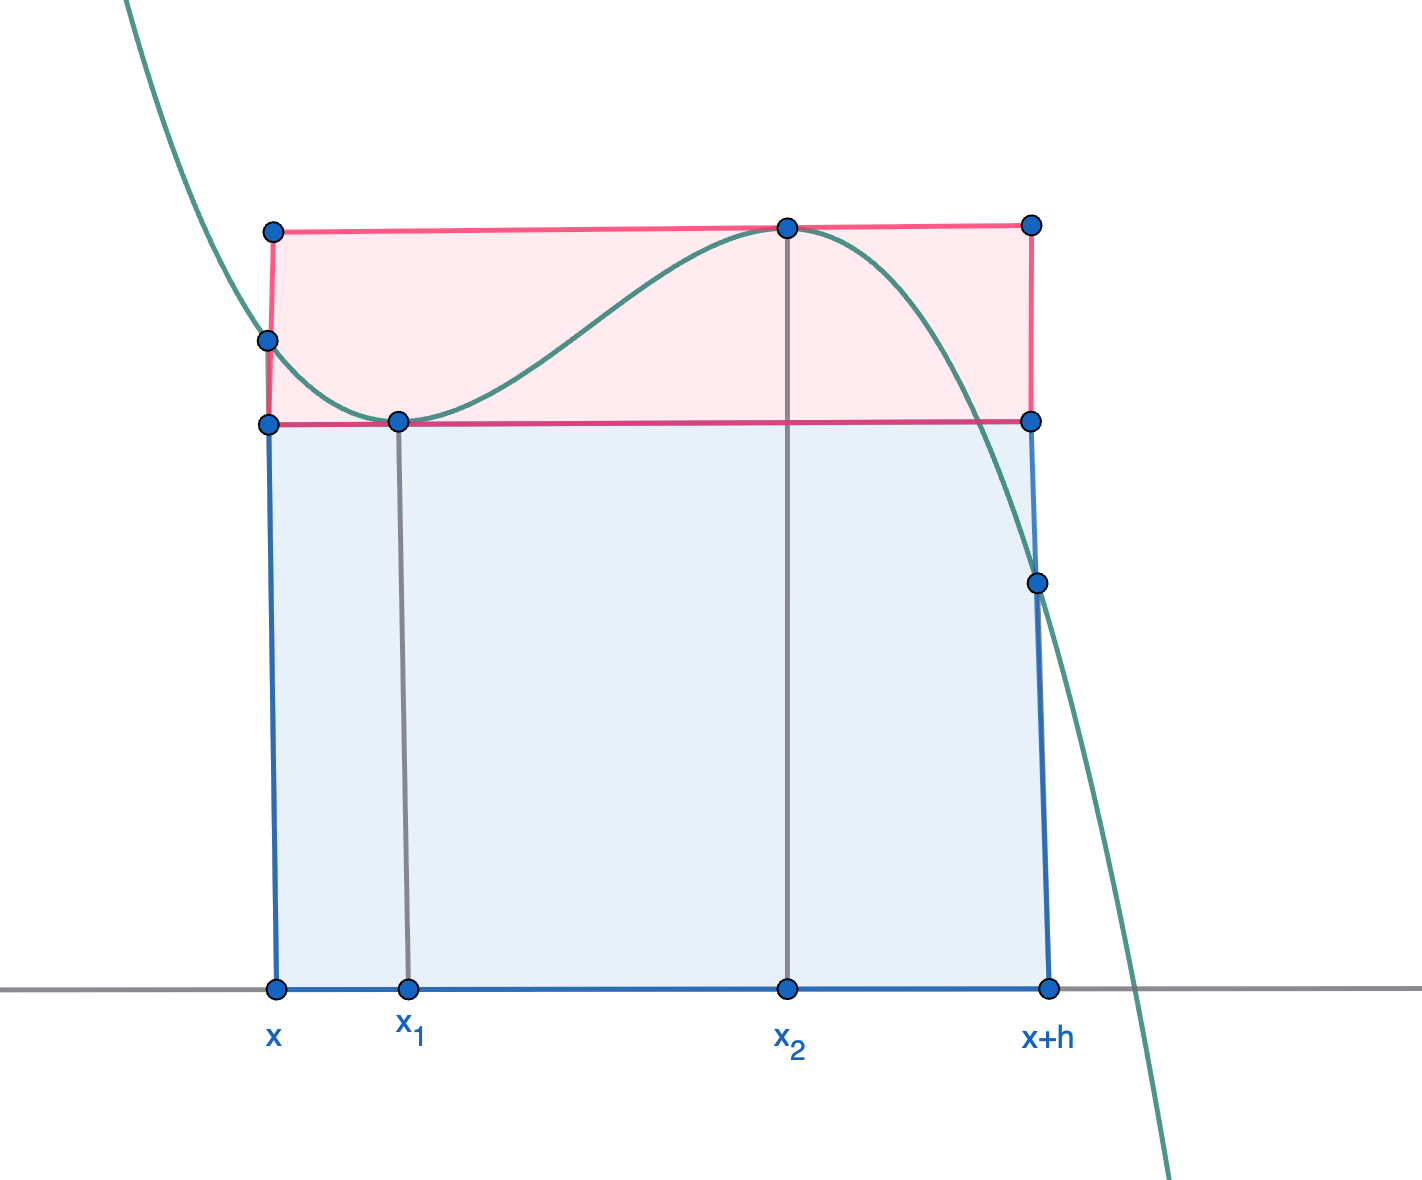
\includegraphics[scale=0.3]{skitser/areal_funktion.png}
\end{figure}

Vi betragter et udsnit af en funktion,
hvor vi ønsker at finde arealet mellem funktionen og $x$-aksen.
Vi antager, at en funktion $A(x)$ giver arealet under grafen indtil $x$-værdien,
og at arealet under grafen på udsnittet ville være givet ved:

$$
    A_{graf}=A(x+h)-A(x)
$$

I udsnittet har vi markeret et interval $x$ til $x+h$,
indenfor dette interval er der et lokalt minimum og maksimum for funktionen.
Arealet under grafen skal være større end eller lig arealet af den blå kasse,
som har længde $h$ og højde $f(x_1)$.
Og arealet skal også være mindre eller lig
arealet af den blå kasse + den røde kasse,
hvilket er den kasse, som har længde $h$ og højde $f(x_2)$.
Derfor kan vi opstille følgende ulighed, som vi kan regne med:

$$
    f(x_1) \cdot h \leq A(x+h)-A(x)
    \leq f(x_2) \cdot h
$$

Først dividerer vi med $h$ på alle sider:

$$
    f(x_1) \leq \frac{A(x+h)-A(x)}{h} \leq f(x_2)
$$

Og så lader vi $h \rightarrow 0$ og deraf:

\begin{align*}
    x_1 &\rightarrow x \\
    x_2 &\rightarrow x \\
    f(x_1) &\rightarrow f(x) \\
    f(x_2) &\rightarrow f(x) \\
    \frac{A(x+h)-A(x)}{h} &\rightarrow A'(x)
\end{align*}

Dette vil sige, at:

$$
    f(x) \leq A'(x) \leq f(x)
$$

Så:
$$
    f(x) = A'(x)
$$

Altså er arealfunktionen af en graf en stamfunktion til funktionen.

\end{proofw}

\section{Integralregning og omdrejningslegeme}

\subsection{Bevis af volumen af omdrejningslegeme}

\begin{proofw}
    
Betragt nedenstående skitse.

\begin{figure}[h]
    \centering
    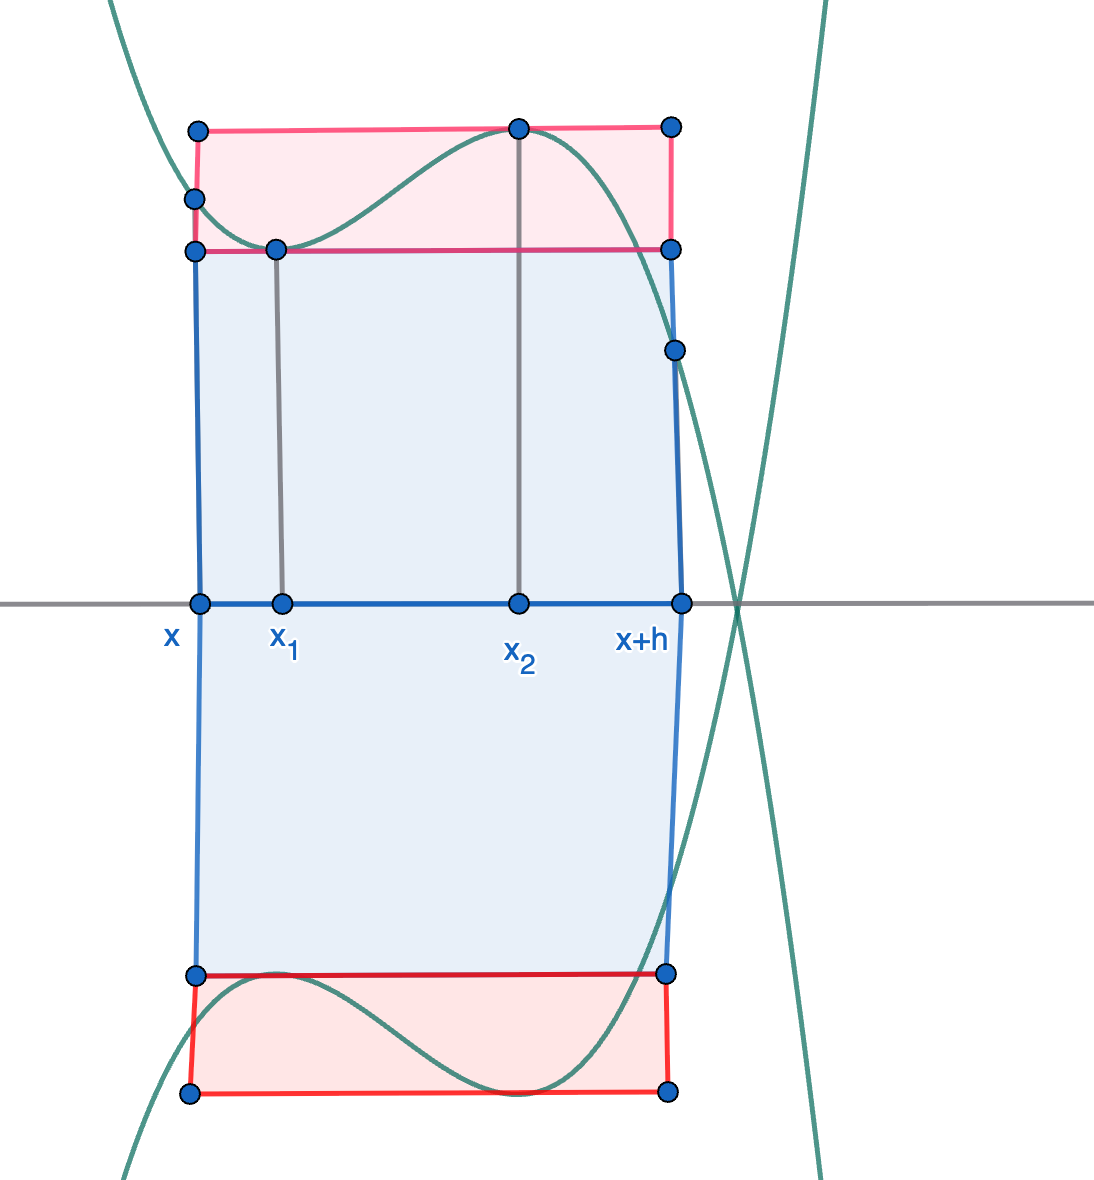
\includegraphics[scale=0.4]{skitser/omdrejningslegeme.png}
\end{figure}

Vi kigger igen på et interval $x$ til $x+h$,
hvor vi er interesserede i volumnet af det omdrejningslegeme,
der fremkommer, når grafen roteres omkring $x$-aksen.
Vi går igen ud fra, at en funktion $V(x)$ giver volumen af omdrejningslegemet
indtil $x$, så volumnet i intervallet er $V=V(x+h)-V(x)$.
Vi antager, at $V(x)$ er differentiabel i intervallet.

Derudover kan vi approksimere volumnet. Som på skitsen
så må der i intervallet være et lokalt minimum og maksimum.
Volumnet må være større eller lig med volumnet af den cylinder,
der har radius $f(x_1)$ og længde $h$, hvis volumen er udtrykt ved:

$$
    V_{min}=h \cdot \pi f(x_1)^2
$$

Omvendt kan volumnet maksimalt være lig med volumnet af cylinderen,
der har højde $f(x_2)$ og længde $h$, hvis areal er:

$$
    V_{max}=h \cdot \pi f(x_2)^2
$$

Nu kan vi opstille følgende ulighed:

$$
h \cdot \pi f(x_1)^2
\leq
V(x+h)-V(x)
\leq
h \cdot \pi f(x_2)^2
$$

Vi deler med $h$:

$$
\pi f(x_1)^2
\leq
\frac{V(x+h)-V(x)}{h}
\leq
 \pi f(x_2)^2
$$

Så lader vi $h \rightarrow 0$, deraf:

\begin{align*}
     x_1 &\rightarrow x \\
    x_2 &\rightarrow x \\
    f(x_1) &\rightarrow f(x) \\
    f(x_2) &\rightarrow f(x) \\
    \frac{V(x+h)-V(x)}{h} &\rightarrow V'(x)
\end{align*}

Så vi får følgende udtryk:

$$
\pi f(x)^2
\leq
V'(x)
\leq
 \pi f(x)^2
$$

Som betyder, at:

$$
V'(x)
=\pi f(x)^2
$$

Vi har vist, at volumen funktionen for det omdrejningslegeme, der fremkommer,
kan findes ved at tage integralet af ovenstående udtryk.

\end{proofw}

\section{Differentialligninger}

\subsection{Bevis af $f$ er løsning til forskudt eksponential vækst}

\begin{proofw}
    Vi skal bevise, at
    $$f(x)=\frac{b}{a}+c\cdot e^{-a \cdot x}$$
    
    er en løsning til differentialligningen:

    $$y'=b-a\cdot y$$

    Først differentierer vi $f$:

    $$
        f'(x)=-a\cdot c\cdot e^{-a\cdot x}
    $$

    Så indsætter vi $f(x)$ i differentialligningen:

    $$
        y'=b-a \cdot \left(\frac{b}{a}+c \cdot e^{-a\cdot x} \right)=b-b+a\cdot c\cdot e^{-a\cdot x}=a\cdot c\cdot e^{-a\cdot x}
    $$

    Så sammenligner vi den differentierede funktion og funktionen indsat i differentialligningen,
    de ser søreme ens ud. Så $f$ er løsning til $y'$.
\end{proofw}

\subsection{Løsning til forskudt eksponential vækst er $f$}

\begin{proofw}
    
Vi vil bevise, at løsningen til 

$$y'=b-a\cdot y$$

er på formen:

$$
    y=\frac{b}{a}+c\cdot e^{-a \cdot x}
$$

Dette gøres ved at indføre en hjælpe funktion $z(x)$ defineret som:

$$
    z(x)=b-a\cdot f(x)
$$

Som vi differentierer:

$$
    z'(x)=-a\cdot f'(x)
$$

Ifølge differentialligningen indsætter vi så $f'(x)=b-a\cdot f(x)$:

$$
    z'(x)=-a\cdot (b-a \cdot f(x))
$$

Hvilket er det samme som $z(x)$, derfor:

$$
    z'(x)=-a\cdot z(x)
$$

Dette er en differentialligning af typen eksponentiel vækst,
hvorved den fuldstændige løsning er givet ved:

$$
    z(x)=c_1\cdot e^{-a\cdot x}
$$

Det betyder, at:

\begin{align*}
    c_1\cdot e^{-a\cdot x}&=b-a\cdot f(x)
    \\
    &\Updownarrow
    \\
    a\cdot f(x)&=b-c_1\cdot e^{-a\cdot x}
     \\
    &\Updownarrow
    \\
    f(x)&=\frac{b}{a}-\frac{c_1}{a}\cdot e^{-a\cdot x}
    \\
    &\Downarrow
    \\
    f(x)&=\frac{b}{a}+c_2\cdot e^{-a\cdot x}
\end{align*}

\end{proofw}

\section{Differentialligninger}

\subsection{Bevis af løsning for logistisk vækst}

\begin{proofw}
    
Vi vil vise den fuldstændige løsning for

$$
    y'=y \cdot (b-a\cdot y)
$$

Hvor løsningen $y \neq 0$.

Først opskriver vi $f$ som differentialligningen:

$$
    f'(x)=f(x) \cdot (b-a \cdot f(x))
$$

Så introducerer vi en hjælpe funktion:

$$
    z(x)=\frac{1}{f(x)}
$$

Som vi differentierer vha. af kædereglen:

$$
    z'(x)=-\frac{1}{f(x)^2} \cdot f'(x)
$$

Her kan vi indsætte differentialligningen:

$$
    z'(x)=-\frac{1}{f(x)^2} \cdot f(x) \cdot (b-a \cdot f(x))
$$

$f(x)$ går ud og vi flytter faktoren op i tælleren:

$$
    z'(x)=-\frac{b-a \cdot f(x)}{f(x)}=\frac{a \cdot f(x)-b}{f(x)}=a-\frac{b}{f(x)}
    =a-b\cdot \frac{1}{f(x)}
$$

Faktoren på $b$ er den samme som $z(x)$, derfor:

$$
    z(x)=a-b\cdot z(x)
$$

Hvilket er en differentialligning for forskudt eksponentiel vækst,
hvis form og løsning er:

\begin{align*}
    y'&=b-a\cdot y
    \\
    y&=\frac{b}{a}+c \cdot e^{-a\cdot x}
\end{align*}

Dette anvendes på differentialligningen for $z$ og husker, at $a$ og $b$ er omvendte:

$$
    z(x)=\frac{a}{b}+c_1 \cdot e^{-b\cdot x}
$$

Så kan vi opstille følgende ligning:

$$
    \frac{1}{f(x)}=\frac{a}{b}+c_1 \cdot e^{-b\cdot x}
$$

Hvor vi isolerer $f(x)$:

$$
    f(x)=\frac{1}{\frac{a}{b}+c_1 \cdot e^{-b\cdot x}}
$$

Denne brøk forlænger vi med $\frac{b}{a}$:

$$
    f(x)=\frac{\frac{b}{a}}{\frac{b}{a} \cdot (\frac{a}{b}+c_1 \cdot e^{-b\cdot x})}
    =\frac{\frac{b}{a}}{
        1+\frac{b}{a}\cdot c_1 \cdot e^{-b \cdot x}
    }
    =
    \frac{\frac{b}{a}}{
        1+c_2 \cdot e^{-b \cdot x}
    }
$$

Derved har vi vist løsningen er på ovenstående form for
en differentialligning på nævnte form.

\end{proofw}

\subsection{Bevis af løsning af logistisk vækst med bærefaktor}

\begin{proofw}
    
Vi vil vise den fuldstændige løsning for 

$$y'=a \cdot y \cdot (M-y)$$

Vi ganger $a$ ind i parentesen:

$$y'=y \cdot (a\cdot M-a \cdot y)$$

Nu har vi faktisk bare en normal logistisk vækst differentialligning,
hvor $b=a \cdot M$, hvis fuldstændige løsning er:

$$
    y=\frac{
\frac{a \cdot M}{a}
    }{
        1+c \cdot e^{-a\cdot M \cdot x}
    }=
    \frac{
M
    }{
        1+c \cdot e^{-a\cdot M \cdot x}
    }
$$

Herved er dette vist.

\end{proofw}

\section{Differentialligninger}

\subsection{Bevis af panserformlen}

\begin{proofw}
    
Vi vil vise den fuldstændige løsning til differentialligningen

$$
    y'+a(x)\cdot y=b(x) \Leftrightarrow y'=-a(x) \cdot y + b(x) 
$$

Vi introducerer en hjælpe funktion $z$:

$$
    z(x)=f(x) \cdot e^{A(x)}
$$

Som vi differentierer, vi udnytter at pga. kædereglen,
så er nedenstående sandt:

$$
    \left(e^{A(x)}\right)'=a(x) \cdot e^{A(x)}
$$

Og vi husker at anvende produktreglen:

$$
    z'(x)=f(x) \cdot a(x) \cdot e^{A(x)}+f'(x)\cdot e^{A(x)}
$$

Vi indsætter differentialligningen og sætter $e^{A(x)}$ udenfor parentes:

$$
    z'(x)= e^{A(x)} \cdot (f(x) \cdot a(x) +f'(x))=
    e^{A(x)} \cdot (f(x) \cdot a(x) +b(x)-a(x)\cdot f(x))
    = b(x) \cdot e^{A(x)}
$$

Da vores afledte kun er bestemt med udtryk af $x$,
så kan vi blot integrere den for at finde stamfunktionen:

$$z(x)= \int b(x) \cdot e^{A(x)} \,dx+c$$

Nu kan vi isolere $f(x)$ fra vores første $z(x)$ udtryk:

$$
    f(x) \cdot e^{A(x)}=\int b(x) \cdot e^{A(x)} \,dx+c
$$

Vi deler med $e^{A(x)}$, hvilket svarer til at gange med $e^{-A(x)}$:

$$
    f(x)=e^{-A(x)} \cdot \int b(x) \cdot e^{A(x)} \,dx+c \cdot e^{-A(x)}
$$

Så er panserformlen bevist.

\end{proofw}

\end{document}
